\chapter{Materials and Methods}
\label{chp:methods}

Introduction to chapter - the chapter contains the following sections
\begin{itemize}
    \item Data collection hardware
    \item Data collection procedures
    \item Post processing of the sensor data
    \item Machine learning methodology
\end{itemize}


%------------------------------------------------------------------%
\section{Data Collection Hardware}
First hand data

What are the requirements for the sensing system - 100Hz, non-intrusive, simple to operate, can be operated on your own

% Sensor selection and location
% Non-invasive wearable sensors, such as Inertial Measurement Units (IMU), are an appealing choice for developing such a system. IMUs give fast update rates, 100s of Hz, are~non-invasive (small with minimal mounting constraints), low cost and have reasonable accuracy. They have been widely used in the field, all of the latest generation of powered prosthetic knees investigated by Fluit et al contained IMUs\cite{Fluit2020}.


\subsection{Movesense Sensor}
The platform chosen for data collection is the Suunto Movesense. This is low cost (£70) \acrfull{cots} device containing a nine-axis \acrshort{imu}/\acrshort{marg} sensor, heart rate monitor, temperature sensor and a \acrfull{ble} radio in a small 10g package. The on-board \acrshort{imu}s sensors are factory calibrated so no additional sensor calibration is required. The device is powered by a small coin cell battery that allows for continuous operation for multiple hours. Figure \ref{fig:methods-movesense-sensor} shows a picture of the Movesense device.

\begin{figure}[!hbt]
    \centering
    \begin{subfigure}[b]{0.4\textwidth}
         \centering
         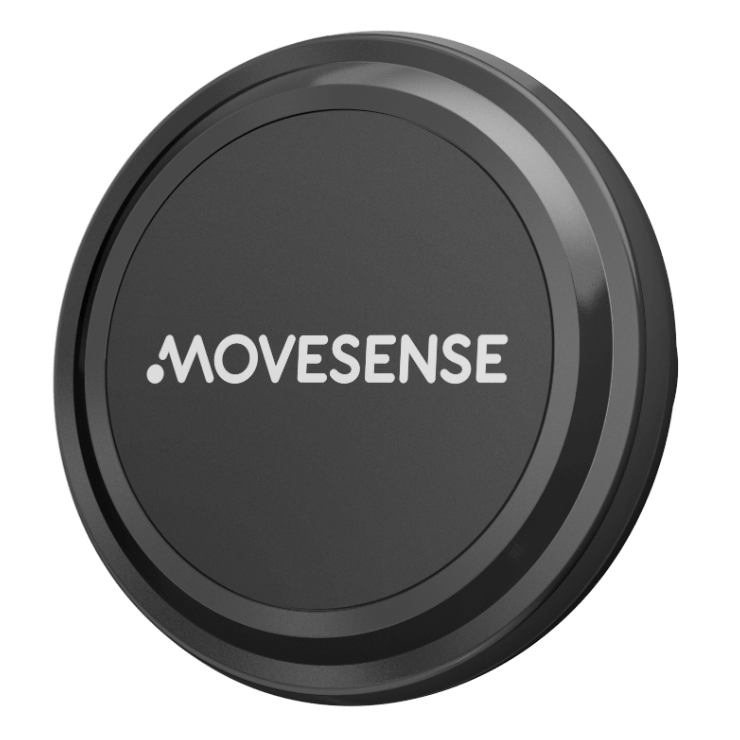
\includegraphics[width=0.9\textwidth]{content/3-Methods/movesense-persp-1000px.png}
    \caption{Front}
    \label{subfig:methods-movesense-sensor}
    \end{subfigure}
    \begin{subfigure}[b]{0.4\textwidth}
         \centering
         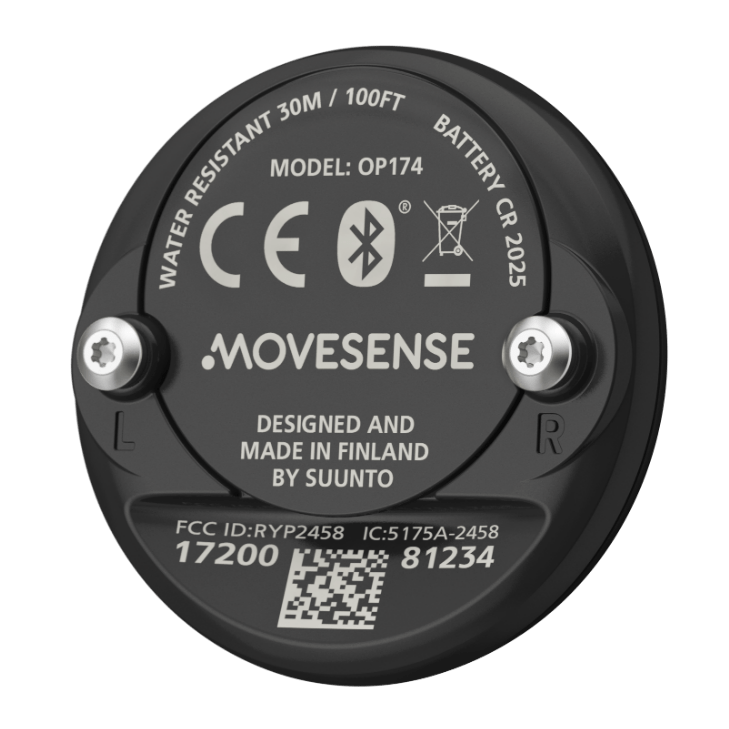
\includegraphics[width=0.9\textwidth]{content/3-Methods/Movesense-rear-1000px.png}
        \caption{Rear}
        \label{subfig:methods-movesense-rear}
    \end{subfigure}
    \caption[Movesense Wearable IMU]{Movesense Wearable IMU \cite{movesenseImg2019}}
    \label{fig:methods-movesense-sensor}
\end{figure}

Custom software can be installed allowing for bespoke setup of the device using the \acrfull{sdk} provided by Suunto. In this software device hardware is accessed through calls to the sensor \acrfull{api}. A custom program was produced that subscribed to the 100Hz \acrshort{marg} output, heart rate and temperature sensor. These were then transmitted over BLE to a android app for data logging. Further details on these steps are presented in subsequent sections.

The software also implemented power management, placing the sensors in a ultra-low power state when inactive, as detected by the accelerometer, for more than 10 minutes. The devices could then be woken again by pressing the rear contacts. This wake interrupt detection is a feature of the on board heart rate monitoring sensors.

The device's rear contact also act as mounting point for attaching the device to a wide variety of sensors. These include heart rate straps and Velcro strap. Five sensors were attached to each participant in the following locations: on the inside of both ankles using an elastic Velcro strap, on~each hip using a clothes/belt clip and across the chest using a heart rate strap. The location of the sensors was selected to give wide coverage of body movements while providing easy, secure and non-invasive attachment to minimize discomfort and disruption to natural movement. Figure~\ref{fig:methods-movesense-sensor-locations} shows a subject wearing the five sensors.

\begin{figure}[!hbt]
    \centering
    \includegraphics[width=0.4\textwidth]{example-image-a}
    \caption{Movesense sensor attachment locations}
    \label{fig:methods-movesense-sensor-locations}
\end{figure}

% How is sensor data transmitted 
\subsubsection{BLE Data Transmission}
\label{subsection:methods-on-sensor-compression}
Data is transmitted wireless using the built in \acrfull{ble} transceiver in the Movesense to a connected smartphone. The process for preparing the sensor data for transmission is presented below.

A custom GATT service was created that allows data packed to be pushed to a connected smartphone. Data pushing is done using the \acrshort{ble} notify mechanism. Data streaming starts when a notify state is set on the \acrshort{ble} characteristic. It stops again when the notify state is cleared. Only enters the high power draw streaming state when recording.

Two limits restrict the data rate that the sensor can transmit. The maximum individual packet size that can be transmitted by the Movesense device is 155 bytes long. There is also a maximum practical transmission rate of less than 15Hz, due to requirements for transmission concurrently from five sensors. The transmission limit require that to achieve a 100Hz sample rate multiple \acrshort{imu} samples are transmitted per packet.

\acrshort{imu} data from the sensor is provided as a 32-bit floating point number. Each sample of the three axis for each of the three sensors requires 36 bytes. At full size only four samples can be packed within the limit for a single BLE transmission. Therefore compression of the data is required.

Compressing the data to 16-bit fixed point signed integer values allow for eight packets of data to be transmitted concurrently. The compression is achieved by multiplying the original value by a scaling factor before typecast to a int-16. This retains the sub-decimal accuracy while allowing for sufficient compression. Table \ref{tab:methods-imu-data-compression-factors} presents the sensor ranges, scaling factors and resultant accuracy of each sensor. As 16-bit integer values have a maximum range of $-32,768$ to $32,767$ clipping would occur if the scaled value of the sensors exceeds this. The scaling factor was therefore chosen as a balance between accuracy and output range with the output range requirement calculated experimentally.

\begin{table}[!hbt]
    \centering
    \caption[Sensor compression scaling factors and accuracies]{Sensor compression scaling factors and accuracies. G --- Force of Gravity, DPS --- Degrees per Second, $\mu T$ --- MicroTesla}
    \label{tab:methods-imu-data-compression-factors}
    
    \begin{tabular}{l|ccc}
         \textbf{Sensor} & \textbf{Sensor Range} & \textbf{Scaling Factor} & \textbf{Accuracy} \\
         \hline
         Acceleromenter & $\pm16 G$ & $256$ & $\pm0.039 G$  \\
         Gyroscope & $\pm2000 DPS$ & $32$ & $\pm0.031 DPS$  \\
         Magnetometer & $\pm5000\mu T$ & $1$ & $\pm1\mu T$
    \end{tabular}
\end{table}

Once compressed 8 IMU samples fit within one packet leaving 11 bytes available. A timestamp based on the internal sensor clock is transmitted as a 32-bit unsigned integer. Six further bytes is populated with the temperature, heart rate and R-R interval recording from the sensor. These were added for future use. As these values are only provided by the sensor on a change in value the remaining byte is used as a update flag for each field. Figure \ref{fig:methods-ble-packet-structure} illustrates the full 155 byte transmission packet.

\begin{figure}[!hbt]
    \centering
    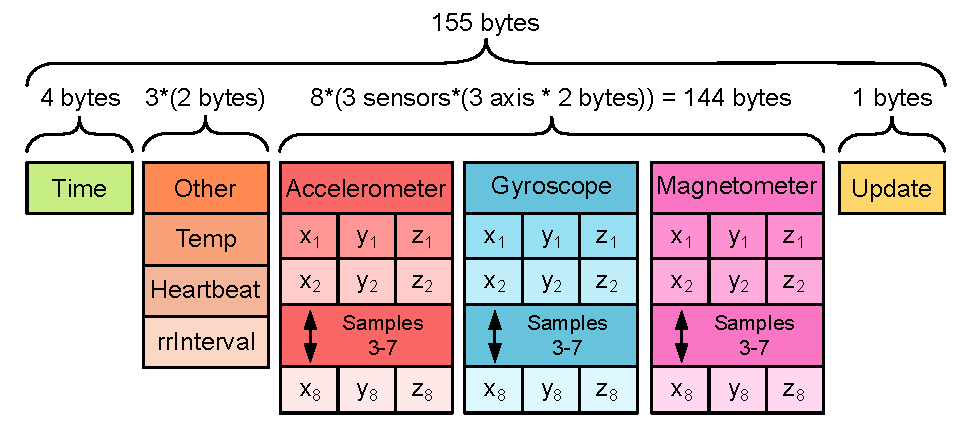
\includegraphics[width=0.9\textwidth]{content/3-Methods/BLE_Bytes_Packets.pdf}
    \caption[Movesense data packet structure]{Movesense Bluetooth Low Energy characteristic transmission packet structure}
    \label{fig:methods-ble-packet-structure}
\end{figure}

\subsection{Android App}
The \acrshort{ble} data stream is received by a smart phone held by the participant. This serves three purposes: to save the sensor data, to annotate the current activity, and to share annotated data with the researcher. These three steps are described in more detail below. 

In recording mode three services run; \acrfull{ui} and \acrshort{ble} and file background services. The \acrshort{ui} service commands the \acrshort{ble} and File services based on user input and also relays information from the two background services to the user. This information includes errors with the sensors and recording statistics. An illustration of the interactions between each aspect of the app is shown in Figure \ref{fig:methods-android-app}.

\begin{figure}[!hbt]
    \centering
    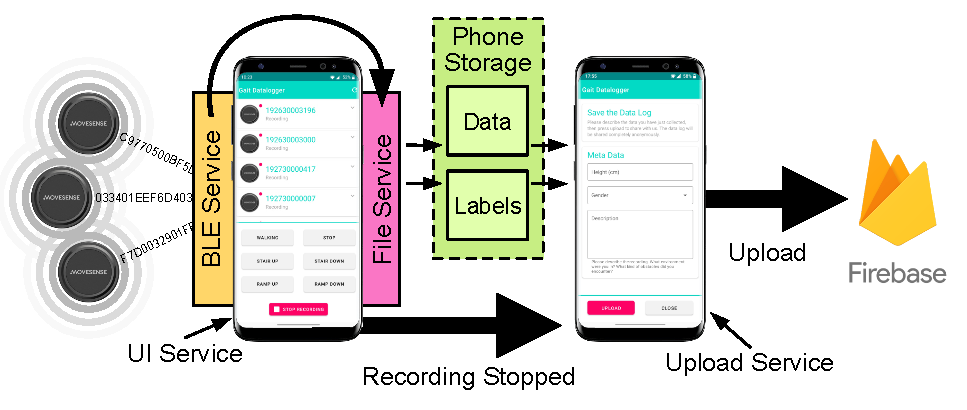
\includegraphics[width=0.9\textwidth]{content/3-Methods/Android_App.pdf}
    \caption{Data-logging Android App}
    \label{fig:methods-android-app}
\end{figure}

\subsubsection{User Interface}
The user interface of the app is intentionally simple requiring minimal instruction to use. The interface is handled by the \acrshort{ui} service. A \acrshort{ble} connection is automatically established with any 'on' sensor that is detected during a \acrshort{ble} device scan when the app opens. If not all sensors are found this search can be repeated.

During recording a series of buttons at the bottom of android app are used to annotate the current activities. Each time a button is pressed the file service records both the name of the button and the phone timestamp to a label file.

Once recording had finished the user is presented with an upload screen allowing metadata to be added and data to be shared with researchers.

\subsubsection{Saving Sensor Data}
The android app is primarily responsible for forming a \acrshort{ble} connection to each sensor and saving the sensor data stream to a file that could be interpreted later. This \acrshort{ble} connection is managed by a background \acrshort{ble} service in the app.

Record is started by the subject pressing the record button. The app then sets the notify state on each device starting data streaming. Received data is passed from the BLE service to the file saving service. This service creates plain text files locally on the phone. Each message of data is saved on a new line in the file along with the phone time stamp and MAC address of the sensor. The data message is saved as a hexadecimal representation of the received binary data string. All sensors are saved together in a single file with each line representing a received BLE data message.

The saved file can then be shared anonymously with the researchers using Google's Firebase cloud services. This uploads the files saved to the phone to google's cloud servers for later retrieval by researchers.

%------------------------------------------------------------%
\section{Data Collection}
\label{sec:methods-data-collection}
First hand data

Introduction and purpose of data collections

%Ethics Approval
The study received ethical approval from the University of Bath Research Ethics Approval Committee for Health (REACH), reference \textit{EP 19/20 003}.

\subsection{Activities}
What activities are we recording. What is the justification for this split

% The following activities were selected, Walking (W), Stair Ascent (SA), Stair Descent (SD), Ramp Ascent (RA), Ramp~Descent (RD) and Stopped (S). Labarri\`ere et al. identified these as the most commonly investigated and they require no equipment or skill to perform~\cite{Labarriere2020}. 

% Pictures showing the variety of terrain %
\begin{figure}[!hbt]
     \centering
     \begin{subfigure}[b]{\textwidth}
         \centering
         \begin{subfigure}[b]{0.32\textwidth}
             \centering
             \includegraphics[width=\textwidth]{example-image-a}
        \end{subfigure}
        \hfill
         \begin{subfigure}[b]{0.32\textwidth}
             \centering
             \includegraphics[width=\textwidth]{example-image-b}
        \end{subfigure}
        \hfill
        \begin{subfigure}[b]{0.32\textwidth}
             \centering
             \includegraphics[width=\textwidth]{example-image-c}
        \end{subfigure}
        \caption{Walking}
        \label{fig:methods-flat-example}
      \end{subfigure}
      \newline
      
      \begin{subfigure}[b]{\textwidth}
         \centering
         \begin{subfigure}[b]{0.32\textwidth}
             \centering
             \includegraphics[width=\textwidth]{example-image-a}
        \end{subfigure}
        \hfill
         \begin{subfigure}[b]{0.32\textwidth}
             \centering
             \includegraphics[width=\textwidth]{example-image-b}
        \end{subfigure}
        \hfill
        \begin{subfigure}[b]{0.32\textwidth}
             \centering
             \includegraphics[width=\textwidth]{example-image-c}
        \end{subfigure}
        \caption{Stairs}
        \label{fig:methods-stair-example}
      \end{subfigure}
      \newline
      
      \begin{subfigure}[b]{\textwidth}
         \centering
         \begin{subfigure}[b]{0.32\textwidth}
             \centering
             \includegraphics[width=\textwidth]{example-image-a}
        \end{subfigure}
        \hfill
         \begin{subfigure}[b]{0.32\textwidth}
             \centering
             \includegraphics[width=\textwidth]{example-image-b}
        \end{subfigure}
        \hfill
        \begin{subfigure}[b]{0.32\textwidth}
             \centering
             \includegraphics[width=\textwidth]{example-image-c}
        \end{subfigure}
        \caption{Ramp/Hill}
        \label{fig:methods-ramp-example}
      \end{subfigure}
    \caption{Example of data recording environments}
    \label{fig:three graphs}
\end{figure}


\subsection{Recording Procedure}
How were the subjects instructed to label data - press at first HS on new activity
% Does this belong here - probably covered by each individual section

% Study subjects were provided with instructions on how to use the sensing equipment, and the activity classes, then~allowed to record as they wished. Participants were instructed to walk around a varied environment with the sensor on while labelling the six activity classes. No~further instructions on how the recording should be conducted were provided.

\subsection{Data-Set Summary} %Should this be part of the materials section?
A brief summary of the data collected over the course of this research is presented in this section. This is followed by a short discussion about the quality of the data.

Data was collected in three phases:
\begin{itemize}
    \item Large number of non-amputee participants - limited data per participant
    \item Small number of non-amputee participants - extensive data per participant
    \item Data from amputees
\end{itemize}
Within this section a brief summary of the data collected is presented.

The first phase of data collection involves collecting a data with a focus of collecting from a broad range of individuals in different environments. Table \ref{tab:methods-phase-1-data-summary} contains a summary of the data collected during the first phase of data collection. Data was collected from twenty-two participants of a wide variety of age (mean 29, std 10), gender (17 male, 5 female), and physique.
\newcolumntype{Y}{>{\centering\arraybackslash}X}
\begin{table}[!hbt]
    \centering
    \caption[Data samples of non-amputee data collected during the first phase of data collection]{Summary of non-amputee data collected during the first phase of data collection.}
    %W---Walking, RA---Ramp Ascent, RD---Ramp Descent, SA---Stair Ascent, SD---Stair Descent, S---Stopped
    \begin{tabularx}{\textwidth}{c|YYYYYY}
       \textbf{Subject ID} & \textbf{W} & \textbf{RA} & \textbf{RD} & \textbf{SA} & \textbf{SD} & \textbf{S} \\
       \hline
       01 & 1111 & 2222 & 3333 & 4444 & 5555 & 6666 \\
       02 & 1111 & 2222 & 3333 & 4444 & 5555 & 6666 \\
       03 & 1111 & 2222 & 3333 & 4444 & 5555 & 6666 \\
       04 & 1111 & 2222 & 3333 & 4444 & 5555 & 6666 \\
       05 & 1111 & 2222 & 3333 & 4444 & 5555 & 6666 \\
       06 & 1111 & 2222 & 3333 & 4444 & 5555 & 6666 \\
       07 & 1111 & 2222 & 3333 & 4444 & 5555 & 6666 \\
       08 & 1111 & 2222 & 3333 & 4444 & 5555 & 6666 \\
       09 & 1111 & 2222 & 3333 & 4444 & 5555 & 6666 \\
       10 & 1111 & 2222 & 3333 & 4444 & 5555 & 6666 \\
       11 & 1111 & 2222 & 3333 & 4444 & 5555 & 6666 \\
       12 & 1111 & 2222 & 3333 & 4444 & 5555 & 6666 \\
       13 & 1111 & 2222 & 3333 & 4444 & 5555 & 6666 \\
       14 & 1111 & 2222 & 3333 & 4444 & 5555 & 6666 \\
       15 & 1111 & 2222 & 3333 & 4444 & 5555 & 6666 \\
       16 & 1111 & 2222 & 3333 & 4444 & 5555 & 6666 \\
       17 & 1111 & 2222 & 3333 & 4444 & 5555 & 6666 \\
       18 & 1111 & 2222 & 3333 & 4444 & 5555 & 6666 \\
       19 & 1111 & 2222 & 3333 & 4444 & 5555 & 6666 \\
       20 & 1111 & 2222 & 3333 & 4444 & 5555 & 6666 \\
       21 & 1111 & 2222 & 3333 & 4444 & 5555 & 6666 \\
       22 & 1111 & 2222 & 3333 & 4444 & 5555 & 6666 \\
    \end{tabularx}
    \label{tab:methods-phase-1-data-summary}
\end{table}

The second phase of data collection involved the collection of data from a much smaller number of individuals but with a focus on collecting at least seven minutes of data for each activity. Table \ref{tab:methods-phase-2-data-summary} show a summary of the data collected during the second phase. Data was collected from two subjects, one male of age 27, and one female of age 26.
\begin{table}[!hbt]
    \centering
    \caption[Data samples of non-amputee data collected during the second phase of data collection]{Data samples of non-amputee data collected during the second phase of data collection}
    \begin{tabularx}{\textwidth}{c|YYYYYY}
       \textbf{Subject ID} & \textbf{W} & \textbf{RA} & \textbf{RD} & \textbf{SA} & \textbf{SD} & \textbf{S} \\
       \hline
       01 & 1111 & 2222 & 3333 & 4444 & 5555 & 6666 \\
       09 & 1111 & 2222 & 3333 & 4444 & 5555 & 6666 \\
    \end{tabularx}
    \label{tab:methods-phase-2-data-summary}
\end{table}

% Third round of data collection
The third range of data collection is amputee data, this involved collecting data with the recording data procedures. Table \ref{tab:methods-phase-3-data-summary} contains a summary of the first hand data collected during this phase. The data was for one trans-tibial amputee.
% Amputee data
\begin{table}[!hbt]
    \centering
    \caption[Data samples of first hand amputee data collected during the third phase of data collection]{Data samples of first hand amputee data collected during the third phase of data collection.}
    \begin{tabularx}{\textwidth}{c|YYYYYY}
       \textbf{Subject ID} & \textbf{W} & \textbf{RA} & \textbf{RD} & \textbf{SA} & \textbf{SD} & \textbf{S} \\
       \hline
       A1 & 1111 & 2222 & 3333 & 4444 & 5555 & 6666 \\
    \end{tabularx}
    \label{tab:methods-phase-3-data-summary}
\end{table}

Additional data was also supplied by the Bio-Mechanics lab of the University of Bath and Blatchford Ltd. Table \ref{tab:methods-second-hand-amputee-data} contains a summary of the additional data obtained during this phase. The data was for \hl{x} trans-tibial and \hl{y} trans-femoral amputees.
% bio-mechanics data of amputee - recap what's different about this data
\begin{table}[!hbt]
    \centering
    \caption[Data samples for other amputee data obtained]{Data samples for other amputee data obtained.}
    \begin{tabularx}{\textwidth}{c|YYYYYY}
       \textbf{Subject ID} & \textbf{W} & \textbf{RA} & \textbf{RD} & \textbf{SA} & \textbf{SD} & \textbf{S} \\
       \hline
       A2 & 1111 & 2222 & 3333 & 4444 & 5555 & 6666 \\
    \end{tabularx}

    \label{tab:methods-second-hand-amputee-data}
\end{table}


What is unique about our data set
\begin{itemize}
    \item Unsupervised (no researcher bias in activity pattern) - subject Provided with sensors, app and basic instructions of how to setup and label data
    \item Wide range of different natural environments and terrain
    \item Large number of people
\end{itemize}

Issues with the data
\begin{itemize}
    \item Poorly distributed classes - real life distribution of activities is not even. Walking and hills/ramps are far more prevalent than stairs - % TODO add in percentage of each activity type for the overall data set and a mean/std per participant 
    \item Transition between activities is inconsistent and only labelled at one point
    \item Label noise
    \item Different amounts of data for different participants
\end{itemize}

%------------------------------------------------------------------%
\section{Data Post-Processing}
The raw saved data must be transformed in order that it can be used in a machine learning environment. Within this sections the methods used to accomplish this transformation are detailed.

% Terminology
The data collected can be described by the following hierarchical structure shown in Figure \ref{fig:methods-data-hierachy}.For each participant a series of data recordings are collected. Each recordings potentially contain different distributions of activities and in different environments. The recording contains a series of activities live annotated by the subject. Each continuous period of one activity label is an episode of data. So a recording is made up of a series of contiguous episodes of data. The period at the end of one episode and start of the next is the transition period between activities. This is represented as a discrete change but in reality would be a smooth easing between locomotive modes.

\begin{figure}[!hbt]
    \centering
    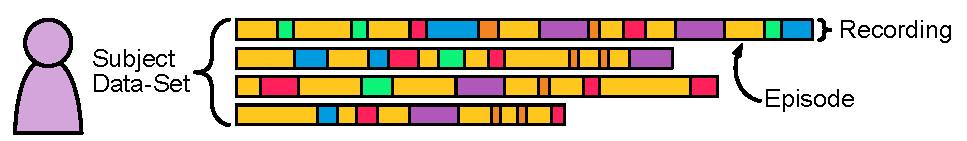
\includegraphics[width=0.9\textwidth]{content/3-Methods/Data_Terminology.pdf}
    \caption{Hierarchical structure of the data recordings and terminology}
    \label{fig:methods-data-hierachy}
\end{figure}

%Issues with the data

    
To prepare the data for \acrshort{ml} and address issues with the data two \acrfull{etl} scripts were written. An \acrshort{etl} is a common technique in data science for copying data from one or more source to a new destination which requires a different representation of the data. A \acrshort{etl} script written in Matlab is used to transform the sensor data from it's saved form to csv files that could easily be imported into a Python. A second \acrshort{etl} script in python then prepare the data for loading into a machine learning environment. A more detailed description of these two scripts is presented in Sections \ref{subsec:sensor-ETL} and \ref{subsec:ML-ETL}

\subsection{Sensor Data ETL}
\label{subsec:sensor-ETL}
The sensor data \acrshort{etl} script transforms the raw saved sensor data into .csv tables that are easily importable into python. Each step of the \acrshort{etl} is described below. The overall process is illustrated in Figure \ref{fig:methods_sensor_ETL}.

\begin{figure}[!hbt]
    \centering
    \includegraphics[width=0.4\textwidth]{example-image-a}
    \caption{Flow Diagram of Sensor Data \acrshort{etl} process}
    \label{fig:methods_sensor_ETL}
\end{figure}

\subsubsection{Extract} % Extract - retrieving data from source
Data is saved in individual directory for each participant and a sub-directory for each recording session. Within each sub-directory three files are store, a data file, label file and meta-data file. The three files contain the following:
\begin{itemize}
    \item \textbf{Data File} -- Hexadecimal encoded binary sensor data along with the mobile phone timestamp at which it was received.
    \item \textbf{Label File} -- Plain text activity labels with timestamps of the activity start (the point at which the app button was pressed)
    \item \textbf{Meta File} -- Notes about the recording including the participant height, gender and a brief unstructured description of the recording.
\end{itemize}

Each sub-directory is opened and processed one at a time in no specified order.

\subsubsection{Transform}
% Transform
The sensor data is store as a Hexadecimal string, with each two characters representing one byte of the transmission string from the sensors. The first operation is converting each pair of characters back into it's original binary value. Then sets of binary values are typecast to integer values before scaling them back into there original 32-bit floating point representation. This is the reverse of the on sensor conversion described in Section \ref{subsection:methods-on-sensor-compression}.

Each line of sensor data contains the Physical/MAC address of the sensor. This is used to split the single file of data into individual sensors. Before combining the individual sensors into a single data table any inconsistency between the devices needs to be accounted for.

The senors do not have on-board real-time clocks the sensor timestamp is based upon their internal clock oscillator. There is sufficient variation between these that clock drift between sensors must be accounted for. To calculate a correction for the long term drift the message timestamp is compared to the smart phone clock. This drift is assumed to be linear therefore a linear regression can be calculated to determine a corrective factor. Figure \ref{fig:methods-clock-drift-correction} shows examples of drift correction. % \hl{}

\begin{figure}[!hbt]
    \centering
    \includegraphics[width=0.4\textwidth]{example-image-a}
    \caption{Example of sensor clock drift correction}
    \label{fig:methods-clock-drift-correction}
\end{figure}

Each data packet contains eight sensors readings, but only one timestamp. Therefore the timestamps for the each individual reading needs to be augmented.

Finally the data is re-sampled to exactly 100Hz to ensure data for each sensors aligns correctly. This was necessary as due to inconsistent sensor clocks the actual device sample rate varies. Re-sampled is performed using the built in Matlab re-sampling function using a spline function to calculate the interpolated value.At this point the individual sensors can be combine into a single data table.

\hl{Normalisation has been shown to improve the performance of ML models}. \cite{} % TODO: find citation
This is performed on a per recording basis maintaining the changes in magnitude that occur when changing between activities. The values for scaling and offset would need to specified on a per user basis for a physical system.

The last step is applying activity labels to the data table. The data labels recorded in the label file are aligned to the recorded data with each row given a label based on the last activity row.

\subsubsection{Load}
Two saving options were employed:
\begin{itemize}
    \item Saving the complete recording as a single file
    \item Splitting the recording up into different files for each episode of an activity
\end{itemize}

The data tables are exported as \acrfull{csv} files, with the \acrshort{csv} files for each participant stored in separate folders. Basic statistics about each file are also generated, including number of samples of each activity and step count.

%--------------------------------------------%
\subsection{Machine Learning ETL}
\label{subsec:ML-ETL}
The second ETL script ingests the \acrshort{csv} data files previously generated and converts and prepares them for loading into a Tensorflow machine learning environment. Tensorflow requires three sets of data, train, test, and validation, each presented as a set of data windows along with a corresponding model output. The \acrshort{etl} script is written in python 3.8. Within this section the process for doing this is presented. A flow diagram of the \acrshort{etl} process is shown in Figure \ref{fig:methods_ml_ETL}.

\begin{figure}[!hbt]
    \centering
    \includegraphics[width=0.4\textwidth]{example-image-a}
    \caption{Flow Diagram of Machine Learning Ingest \acrshort{etl} process}
    \label{fig:methods_ml_ETL}
\end{figure}

% Export
\subsubsection{Extract}
The extract process starts by importing the \acrshort{csv} files using the Python library Pandas. Using Pandas the \acrshort{csv} data is loaded into Pandas data tables and stored against it's associated participant and where applicable activity.

The \acrshort{etl} script also accepts a set of \acrshort{yaml} parameter files. Within these files the parameters for configuring the various transformations are stored. This allow experiments to be replaced quickly as the \acrshort{yaml} files can be stored with the input data and results. The \acrshort{etl} script also supports a \acrshort{yaml} file that specifies a range of values of a single or multiple parameters to test. This allows the \acrshort{etl} script to implement hyper-parameter sweeping.


\subsubsection{Transform -- Data Division}
%The data set was divided into two groups for test and training. The training set was used during the learning process with the test set reserved for evaluating the performance of unseen data. The test set was a variation of Leave One Out Cross-Validation (LOOXV). LOOXV involves training and analyzing the model multiple times with different excluded individuals, the results are then combined to improve statistical certainty. For this paper four/five subjects were excluded each time with analysis repeated five time, meaning each subject was excluded once. The training set contains the remaining subjects, with 30% of the data used as a validation set. Figure 9 provides an illustration of how the data is divided between the three data sets.

%To balance the data set, both the training and test sets were adjusted by removing data so that no class contained more than 50\% more samples than any another. This re-balancing was undertaken carefully so that during validation splitting the balance was maintained. A class weight input was used to bias the training to further balance the class labels.

%The continuous sensor data was segmented using sliding windows. Between the start of each window, an offset of five samples was used. This offset was set empirically to give the model a wide range of data windows position without slowing down learning from an unnecessarily large training set. The output label for each window was set as the recorded ground truth at the end of the window. Classification labels were presented using one-hot encoding.


What are the issues with our data set - primarily that it is poorly distributed. Can be fixed by truncating the dataset or by biasing the training algorithm (class weights).

Aims of division - cross validation + maximise use of relatively small available data / fix issues with the dataset.

Split into training, validation, test. Recap the needs of each of these datasets. Training is as broad a set of data as possible. Validation is a set data drawn out of the training set used to evaluate the training performance. Test should be an independent set of data with the same distribution as the training set. It must be unseen to the training algorithm.

Two methods have been used for dividing the data. The first splits the data by test subject, the second splits the data by activity episodes.

\paragraph{Per Participant Division}
\label{par:methods-per-participant-division}
Split on a per participant basis - natural division point for a group of people

Shuffled to provide a large number of different training and test sets

Limitations of this method
 - How did we accommodate different amounts of data per participant
 
Figure \ref{fig:methods-per-participant-division}
 
 \begin{figure}[!hbt]
     \centering
     \includegraphics[width=0.6\textwidth]{example-image-a}
     \caption{Per-participant data division}
     \label{fig:methods-per-participant-division}
 \end{figure}

\paragraph{Per Episode Division}
\label{par:methods-per-episode-division}
Can't easily split up data per participants due to poor distribution of classes. 

Figure \ref{fig:methods-per-episode-data-division} illustrates the process of forming the three data sets.
For experiments where only an individual participant is available split bases on 'episodes' of data

Episodes are all different lengths so how were episodes combined into test and training sets
    - combine episodes until a threshold is reached. Use remaining data as test set

Limitations of this method
 - Can end up with similar episodes in test and training (data shuffled and cross validation repeated multiple times)
 - Removes transitions from the data set (data is cleaner)
 
 Talk about under/over/mislabelling (Particularly around transitions). How did we account for these? Figure \ref{fig:methods-per-episode-data-division}
 
 \begin{figure}[!hbt]
     \centering
     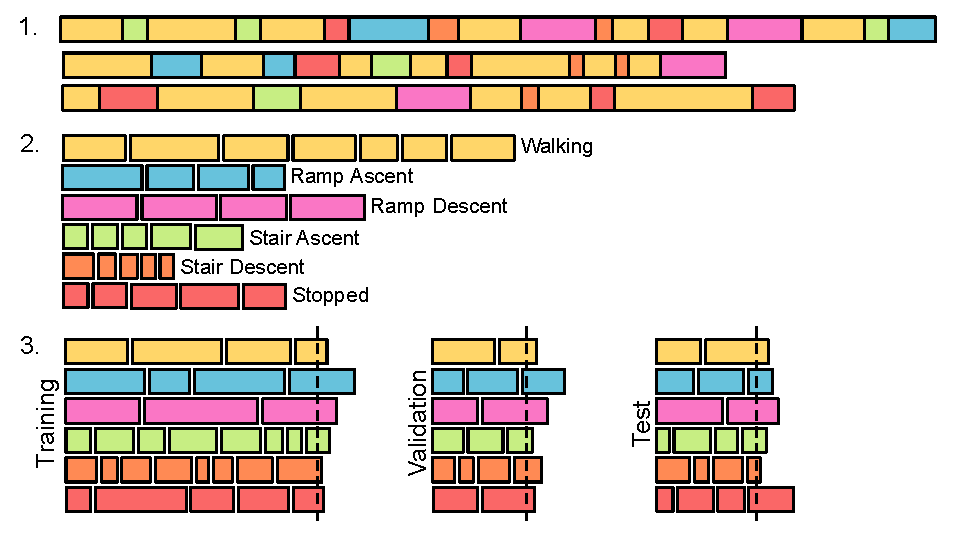
\includegraphics[width=0.9\textwidth]{content/3-Methods/Episode_Division.pdf}
     \caption[Per-episode data division]{Per-episode data division. Step 1 -- All data files for a participant are loaded and labeled. Step 2 -- Episodes of the same activity are grouped together. Step 3 -- Training, Validation and Test sets are formed by stacking episodes until a threshold is reached.}
     \label{fig:methods-per-episode-data-division}
 \end{figure}
 
 
\subsubsection{Transform -- Data Windowing}
The \acrshort{yaml} setup file specify the columns of data that are required, for example \textit{right-ankle-gyro-y}. The data columns specified are extracted from the Pandas data tables with the remaining data columns discarded.

To generate the data windows rows of data equal to the specified window size are selected and copied to form new Pandas data tables. This starts at the beginning of the data table with the starting index incremented forward by a specified step size for each new window. This results in a set of overlapping windows. Figure \ref{fig:methods-data-window-generation} illustrates the data window generation.

\begin{figure}[!hbt]
    \centering
    \includegraphics[width=0.6\textwidth]{example-image-a}
    \caption{Overlapping data window generation}
    \label{fig:methods-data-window-generation}
\end{figure}

The activity labels must be provided in the same output scheme as the \acrshort{ml} model, for classification format called a one-hot encoding in used. This gives each class a separate output with the classification given to the output with the highest value. The activity labels will be presented as an array of length equal to the number of activities. Each element of the array represents one of the activity classes. The class the label represents in encoded by setting the corresponding array element to a value of one.

%In Human Activity Recognition datasets, we note that the samples produced by the same subjects are likely to be correlated due to diverse factors. Hence, k-fold cross validation may overestimate the performance of activity recognizers, in particular when overlapping sliding windows are used. In this paper, we in- vestigate the effect of Subject Cross Validation on the performance of Human Activity Recognition, both with non-overlapping and with overlapping sliding windows. Results show that k-fold cross validation artificially increases the performance of recognizers by about 10\%, and even by 16\% when overlapping windows are used. In addition, we do not observe any performance gain from the use of overlapping windows. We conclude that Human Activity Recog- nition systems should be evaluated by Subject Cross Validation, and that overlapping windows are not worth their extra computational cost.\cite{Dehghani2019}


\subsubsection{Load}
Push into Tensorflow model

Group weights?


%------------------------------------------------------------------%
\section{Machine Learning Methods}
The central challenge in machine learning is that it our algorithm must perform well on new, previously unseen inputs. The ability to perform well on previously unobserved inputs is called generalisation.
What separates machine learning from optimisation is that we want the generalisation error to below as well as the training error.\cite{Goodfellow2015}

\subsection{Model Setup}
Python 3.7
Tensorflow 2.1
Computer specs

% Two different model architectures were developed, a simplified model with a single information path for investigating LSTM internal behavior; and a full complexity practical model based on the architecture presented by Murad et al. [11] for investigating hyperparameter sensitivities. This design was previously discussed in Section 2.2. For both architectures input data is fed directly into the first LSTM layer. For models with additional LSTM layer, the full output of the first LSTM layer is fed into input of the next layer and so on. The output from the final LSTM layer is fed into a fully connected dense layer followed by a ReLU classifier. For the simplified model the LSTM output is the last timestep only, for the full complexity model the full output of all timesteps is used. The size of the dense layer is equal to the number of outputs from the last LSTM layer. A one-hot classification output is used to encode the activity classes. Figure 8a,b show the architectures of the simplified and full complexity model, respectively.


\subsection{Model Training}
%The models were trained to minimize categorical cross-entropy. Model weights were initialized with a Golorot Uniform initializer [43] and optimized with an ADAM optimizer [44]. A dropout of 0.5 was used, selected experimentally, with network connections dropped between the last LSTM output and the dense classifier. During trained the full training dataset was used for each epoch, with data passed to the optimizer in mini batches of 2000 windows. At the end of each epoch the entire validation set was evaluated. Early stopping was used to prevent over-fitting, this stopped training when stagnation of validation cross-entropy loss was observed. Stagnation was identified by three consecutive losses of greater than the minimum previously seen. The model was trained on a PC with an AMD Ryzen 3600 CPU and a Nvidia Geforce RTX 2060 Super. Using GPU training, each epoch took approximately 10 s with between30 and 100 epochs required to train each model depending on the model size and the number of output classes.

hyper parameter sweeping

The test set - composed of examples coming from the same distribution as the training set, can be used to estimate generalisation error of a learner, after the learning process has completed.\cite{Goodfellow2015}

Training set is formed of data used 
Validation set is formed by part of the training set

The validation set error will underestimate the generalisation error, though typically by a smaller amount that the training error. The generalisation error may be estimated using the test set.\cite{Goodfellow2015}

\subsection{Performance analysis}
Accuracy

Confusion matrices
%Miss-classification will be analyzed using confusion matrices. A confusion matrix is a tabular representation of the performance of a classifier. Each cell is populated by a count of the ground truth against the classified output. This allows the accuracy of individual classes and confusion between classes to be assessed.

Precision - What proportion of positive identifications was actually correct? (A model that produces no false positives has a precision of 1.0.)

$p = \frac{TP}{TP + FP} $

Recall - What proportion of actual positives was identified correctly? (A model that produces no false negatives has a recall of 1.0.)

$r = \frac{TP}{TP + FN}$

F1-Score
% EOF
